\subsection{Prodotto realizzato}
\label{subsec:prodotto-realizzato}

Nella {\hyperref[fig:login]{Figura 3.9}} è possibile vedere La pagina di \textit{login}, che consente agli utenti di accedere inserendo le proprie credenziali.\\
In caso di problemi, è disponibile un'opzione per reimpostare la \textit{password} cliccando su "\textit{Password} dimenticata".
\begin{figure}[H]
    \centering
    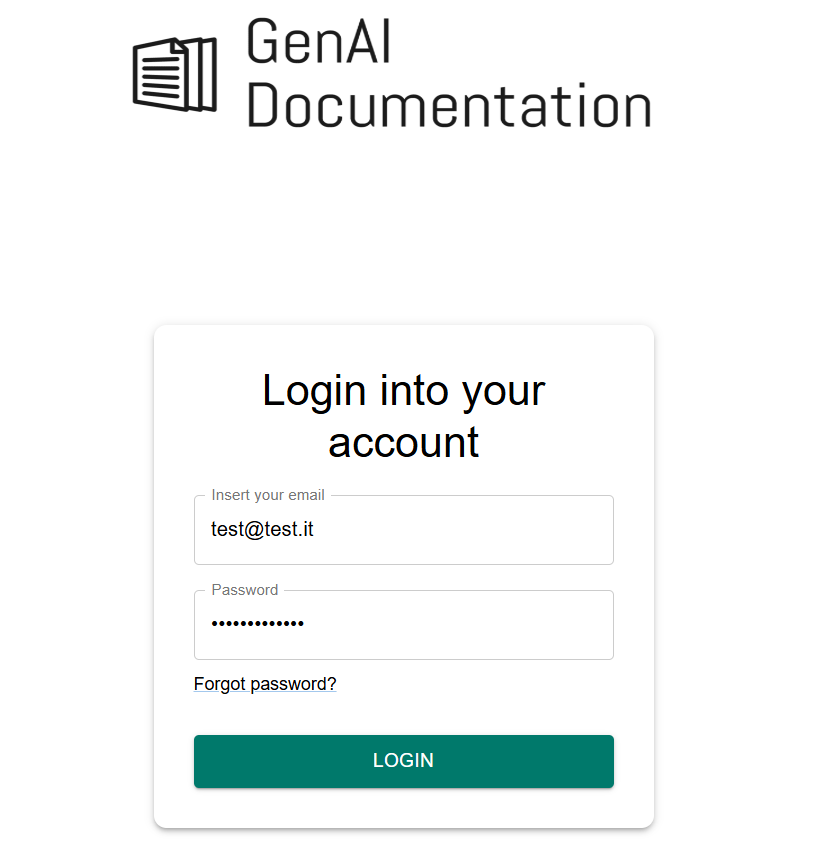
\includegraphics[width=1\textwidth]{applicazione/login.png}
    \caption{Schermata di \textit{login} del progetto}
    \label{fig:login}
\end{figure}

\pagebreak
\noindent La \textit{dashboard}, mostrata in {\hyperref[fig:dashboard]{Figura 3.10}}, offre una panoramica dei progetti generati in precedenza e delle bozze di progetto, con la funzionalità, sia dei progetti che per le bozze,
di cercarle per nome o filtrarle per data. \\
Da questa pagina, gli utenti possono accedere ai dettagli di un singolo progetto o iniziare la generazione di un nuovo progetto, oltre che effettuare il \textit{logout}.\\
\begin{figure}[H]
    \centering
    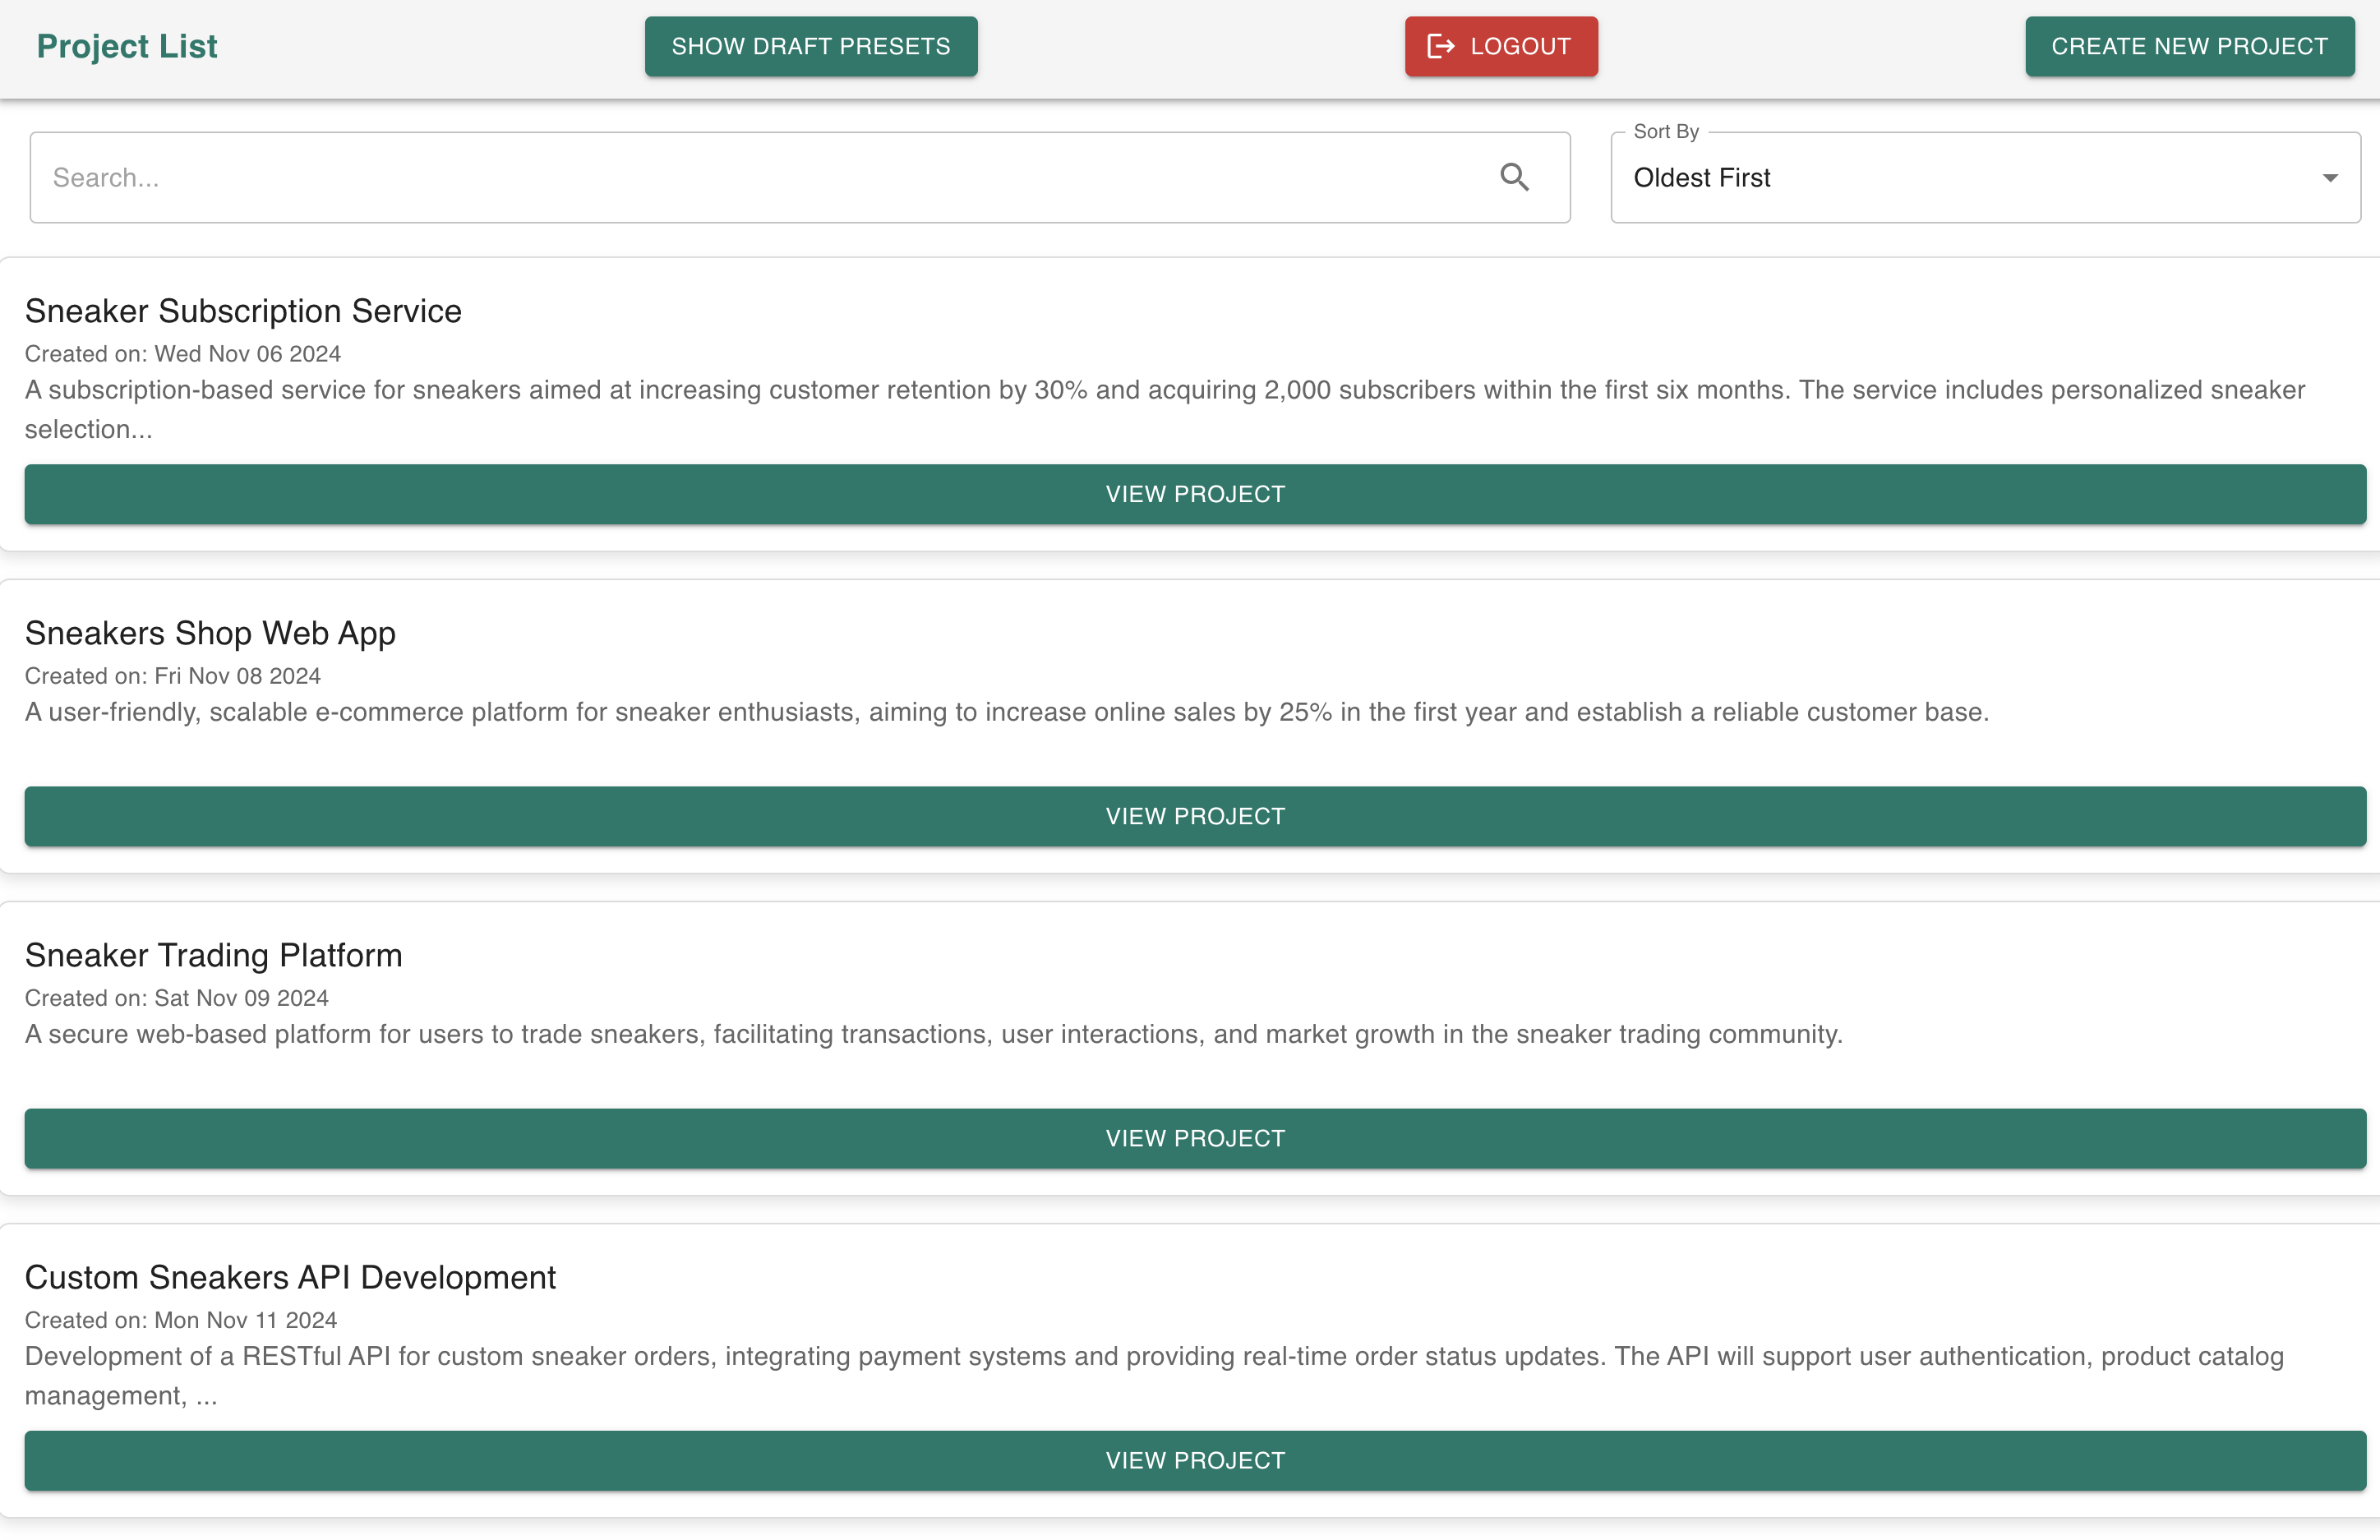
\includegraphics[width=1\textwidth]{applicazione/dashboard.png}
    \caption{Schermata della \textit{dashboard} del progetto}
    \label{fig:dashboard}
\end{figure}

\pagebreak
\noindent In {\hyperref[fig:create-project]{Figura 3.11}} è possibile vedere la pagina di generazione di un progetto permette di creare nuovi progetti inserendo il nome, selezionando un \textit{preset} e completandolo in tutte le sue sezioni.\\
Una volta compilato, l’utente può procedere con la generazione del progetto. \\
È inoltre possibile salvare il \textit{preset} parzialmente compilato come bozza per riprenderlo in un secondo momento.
\begin{figure}[H]
    \centering
    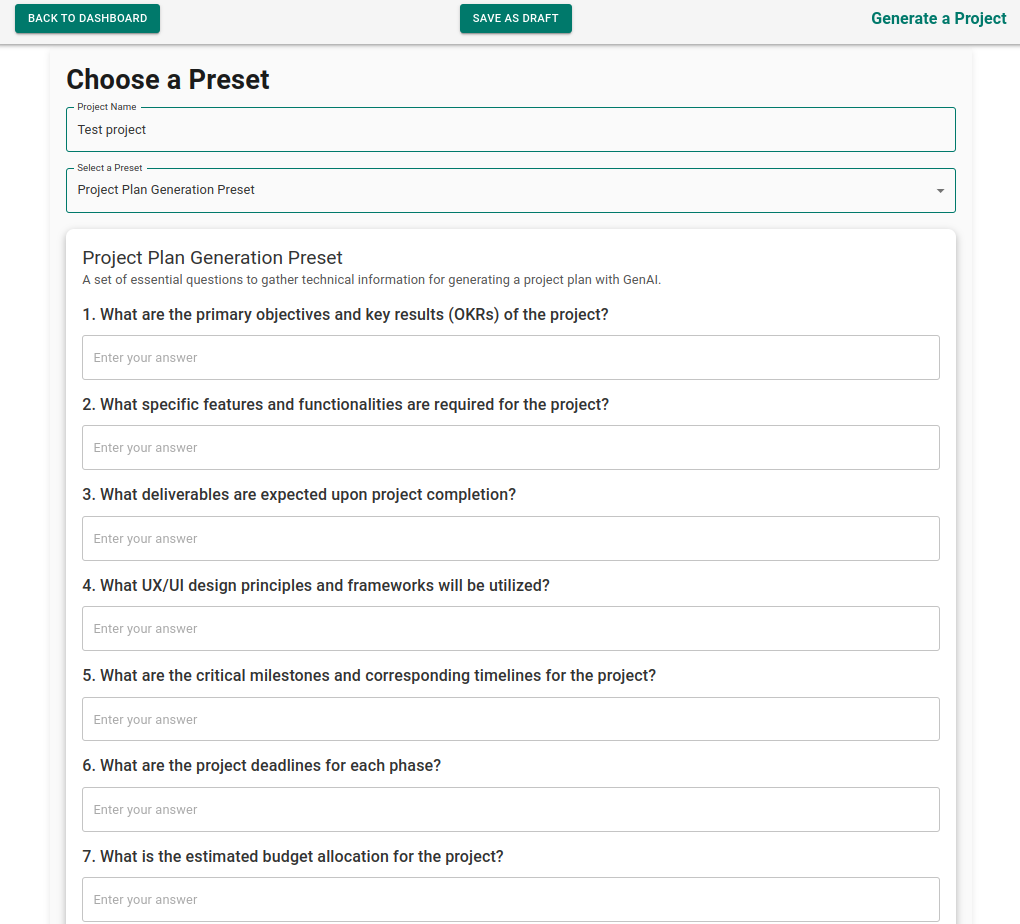
\includegraphics[width=1\textwidth]{applicazione/create-project.png}
    \caption{Schermata di generazione del progetto}
    \label{fig:create-project}
\end{figure}

\pagebreak
\noindent In {\hyperref[fig:project-detail]{Figura 3.12}} è possibile vedere la pagina di visualizzazione di un singolo progetto offre una panoramica completa di tutte le informazioni relative al progetto, inclusi i dettagli tecnici ed il PDF generato, che può essere visualizzato direttamente nella pagina. \\ 
Gli utenti possono scegliere di rigenerare l’intero progetto oppure focalizzarsi su una singola sezione, utilizzando una finestra che consente di inserire un \gls{prompt} personalizzato, come mostrato in {\hyperref[fig:regenerate-project]{Figura 3.13}}.\\
\begin{figure}[H]
    \centering
    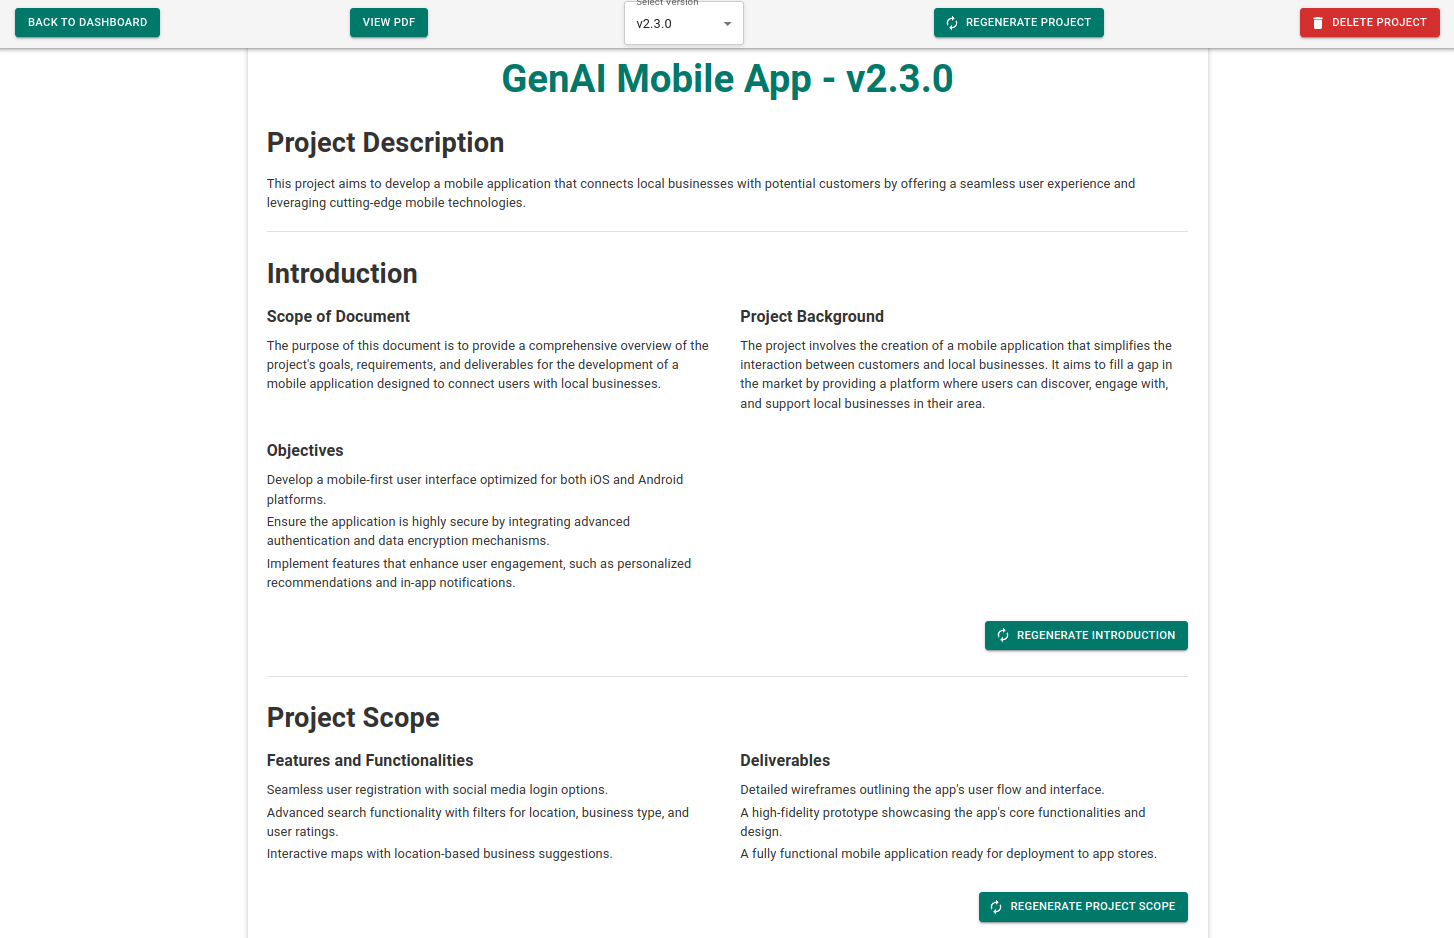
\includegraphics[width=1\textwidth]{applicazione/project-detail.png}
    \caption{Schermata di dettaglio del progetto}
    \label{fig:project-detail}
\end{figure}

\begin{figure}[H]
    \centering
    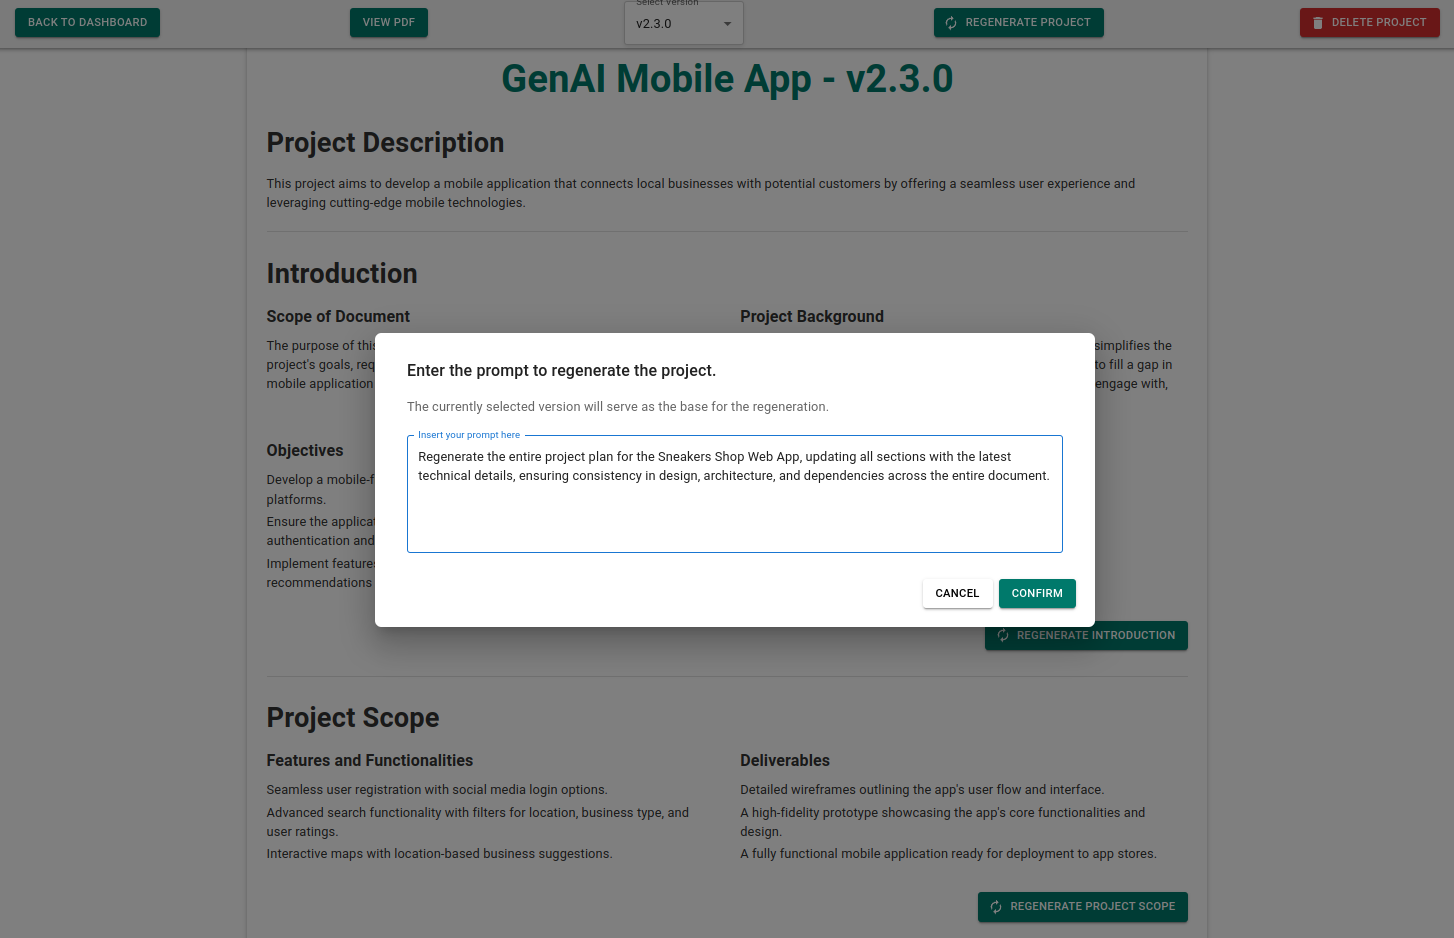
\includegraphics[width=1\textwidth]{applicazione/regenerate-project.png}
    \caption{\gls{prompt} per rigenerare il progetto}
    \label{fig:regenerate-project}
\end{figure}

\pagebreak
\noindent In {\hyperref[fig:swagger]{Figura 3.14}} è possibile vedere La lagina di visualizzazione del \textit{Swagger} delle \gls{api} fornisce una documentazione interattiva e dettagliata delle \gls{api} disponibili nel sistema. \\
Attraverso questa pagina, gli utenti possono esplorare i vari \textit{endpoint}, visualizzarne le descrizioni, i parametri richiesti e le risposte previste. \\
Inoltre, è possibile effettuare chiamate di prova direttamente dalla pagina, inserendo i parametri necessari e verificando i risultati in tempo reale. 
\begin{figure}[H]
    \centering
    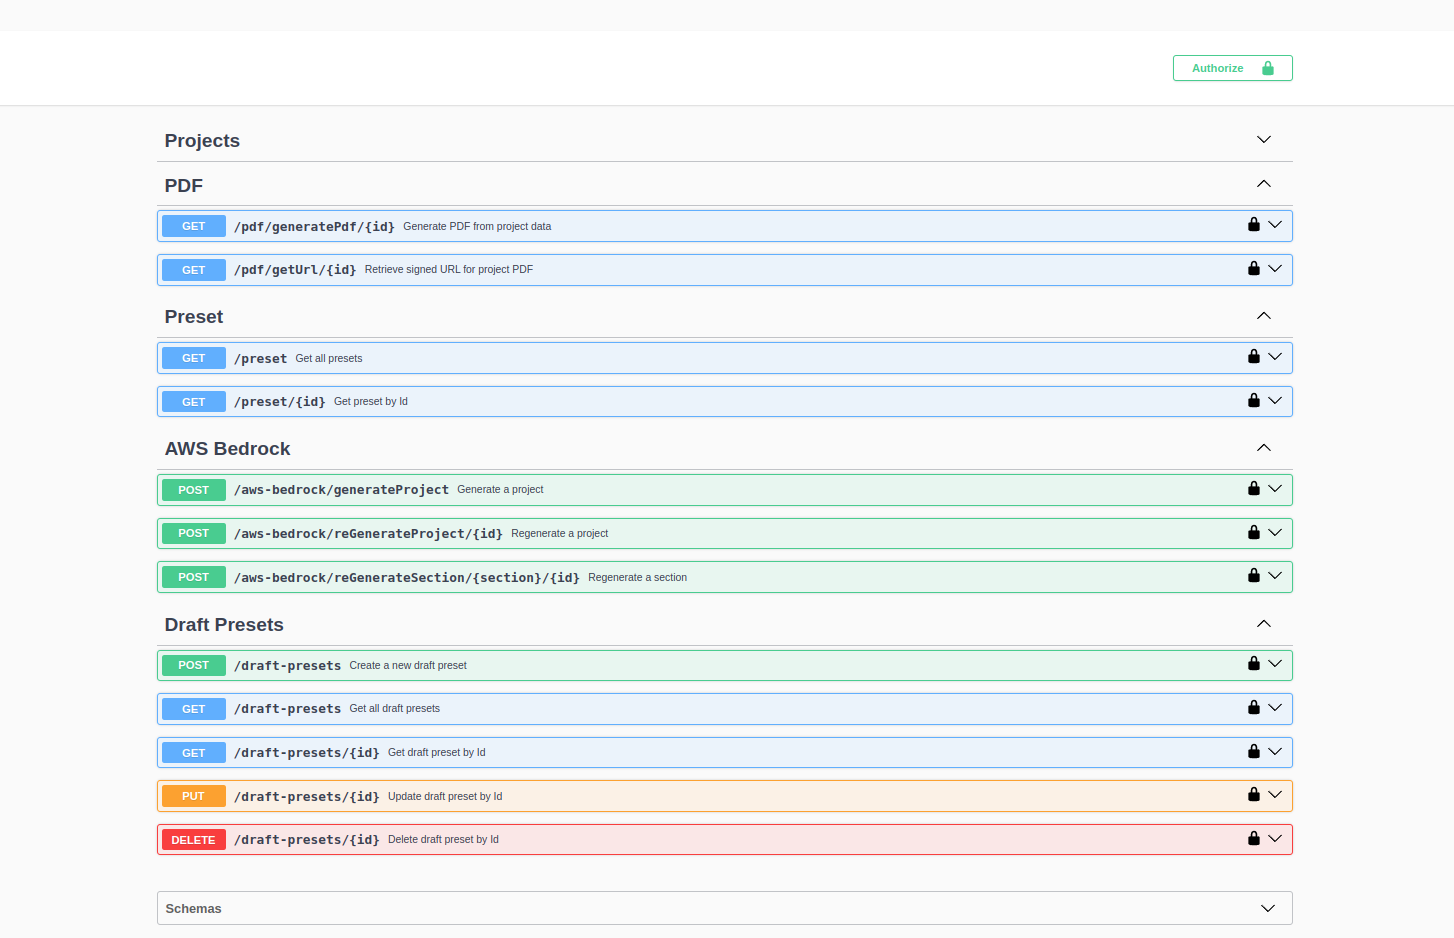
\includegraphics[width=1\textwidth]{applicazione/swagger.png}
    \caption{\textit{Swagger} delle \gls{api} create}
    \label{fig:swagger}
\end{figure}